\begin{frame}{music ai}{where we are now}
    \vspace{-3mm}
    \begin{center}
        \begin{tabular}{cccc}
            \includeaudio{RobotBlues} &
            \includeaudio{FunkyFuture} &
            \includeaudio{RiseMachines} &
            \includeaudio{StolenStrings}\\
            blues & funk & metal & chanson\footnote{generated on suno.com with the same prompt for different genres}
        \end{tabular}
    \end{center}

    \begin{itemize}
        \item   ML/AI used by and \textbf{impacting all stakeholders} in chain of music communication
            \begin{itemize}
                \item content creators
                \item   performers
                \item   producers
                \item   labels/music industry
                \item   distributors
                \item consumers
            \end{itemize}
        \item   technologies are \textbf{here to stay} 
        \item technologies \textbf{will improve} in usability, reliability, and accuracy
    \end{itemize}
    %\begin{columns}
    %\column{.5\linewidth}{\textbf{opportunities}}
    %
        %\begin{itemize}
            %\item content creation:
                %\begin{itemize}
                    %\item speed-up, increased efficiency
                    %\item creative possibilities (morphing, etc.)
                    %\item co-creative idea givers
                    %\item democratization
                %\end{itemize}
            %\smallskip
            %\item consumption:
                %\begin{itemize}
                    %\item personalization
                    %\item effective discovery and accessibility
                    %\item (inter)active listening experiences
                %\end{itemize}
        %\end{itemize}
    %\column{.5\linewidth}{\visible<2->{\textbf{threats}}}
    %
        %\begin{itemize}
            %\item<2-> content creation:
                %\begin{itemize}
                    %\item ethical use of data
                    %\item growth in plagiarism
                    %\item liability for harmful content
                    %\item livelihood of  creators
                    %\item value perception of artistic content
                %\end{itemize}
            %\smallskip
            %\item<2-> consumption:
                %\begin{itemize}
                    %\item consumer distrust through 
                        %\begin{itemize}
                            %\item inflationary ai-generated content
                            %\item inexplainable black-box systems
                        %\end{itemize}
                %\end{itemize}
            %\item<2-> both:
                %\begin{itemize}
                    %\item 'mainstreamification'
                    %\item bias (data curation, for-profit system control)
                    %\item sustainability and energy 
                %\end{itemize}
        %\end{itemize}
        %\vspace{20mm}
        %\begin{figure}%
            %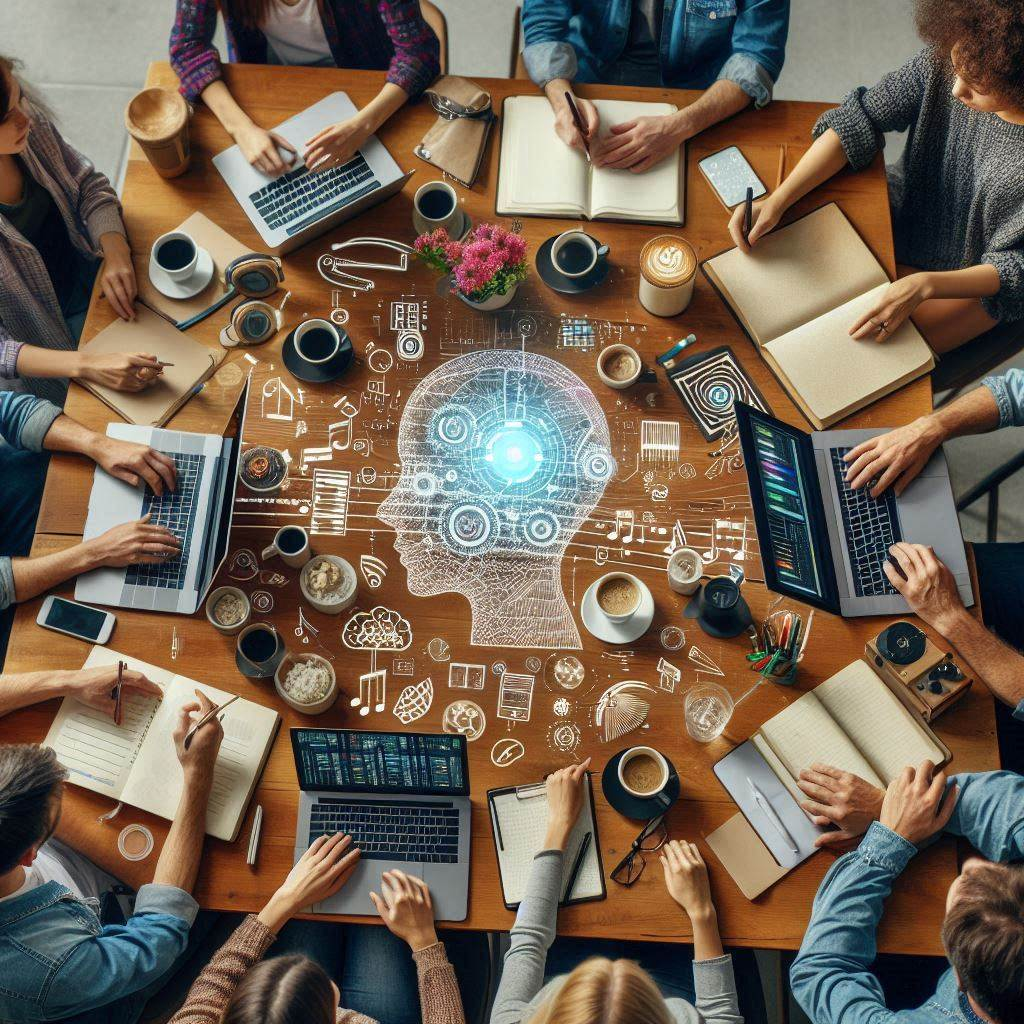
\includegraphics[width=.8\columnwidth]{responsible-ai}%
        %\end{figure}
    %\end{columns}
    \inserticon{../musicdata}
\end{frame}


\begin{frame}{music ai}{opportunities}

    \begin{columns}
    \column{.65\linewidth}
        \begin{itemize}
        \item \textbf{content creation, production}:
                \begin{itemize}
                \item increased efficiency
                \item expanded creative options (separation, morphing, etc.)
                \item co-creative idea generation
                \item democratization of music making
                \end{itemize}
        \bigskip
            \item \textbf{consumption}:
                \begin{itemize}
                    \item personalization
                    \item effective discovery and accessibility
                    \item (inter)active listening experiences
                \end{itemize}
        \end{itemize}
    \column{.35\linewidth}
        \begin{figure}
            \vspace{13mm}
            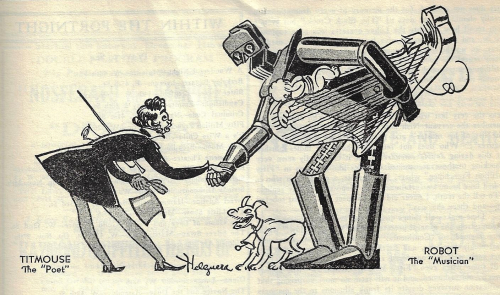
\includegraphics[scale=.7]{graph/musical-robots}
        \end{figure}
        \addreference{\href{https://longstreet.typepad.com/thesciencebookstore/2017/06/the-invasion-of-musical-robots-1929.html}{longstreet.typepad.com/thesciencebookstore/2017/06/the-invasion-of-musical-robots-1929.html}}
    \end{columns}

\end{frame}


\begin{frame}{music ai}{risks \& threats}
    \vspace{-7mm}
    \begin{columns}
    \column{.65\linewidth}
        \begin{itemize}
            \item \textbf{content creation, production}:
                \begin{itemize}
                    \item ethical use of data
                    \item growth in plagiarism, impersonation
                    \item liability for harmful content
                    \item livelihood of  creators
                    \item value perception of artistic content
                \end{itemize}
            \smallskip
            \item<2-> \textbf{consumption}:
                \begin{itemize}
                    \item consumer distrust through 
                        \begin{itemize}
                            \item inflationary ai-generated content
                            \item inexplainable black-box systems
                        \end{itemize}
                \end{itemize}
            %\smallskip
            \item<3-> \textbf{general}:
                \begin{itemize}
                    \item 'mainstreamification' (novelty vs.\ homogeneity)
                    \item bias (data curation)
                    \item monopolization (for-profit system control)
                    \item sustainability and energy 
                \end{itemize}
        \end{itemize}
    \column{.35\linewidth}
        \begin{figure}
            \vspace{10mm}
            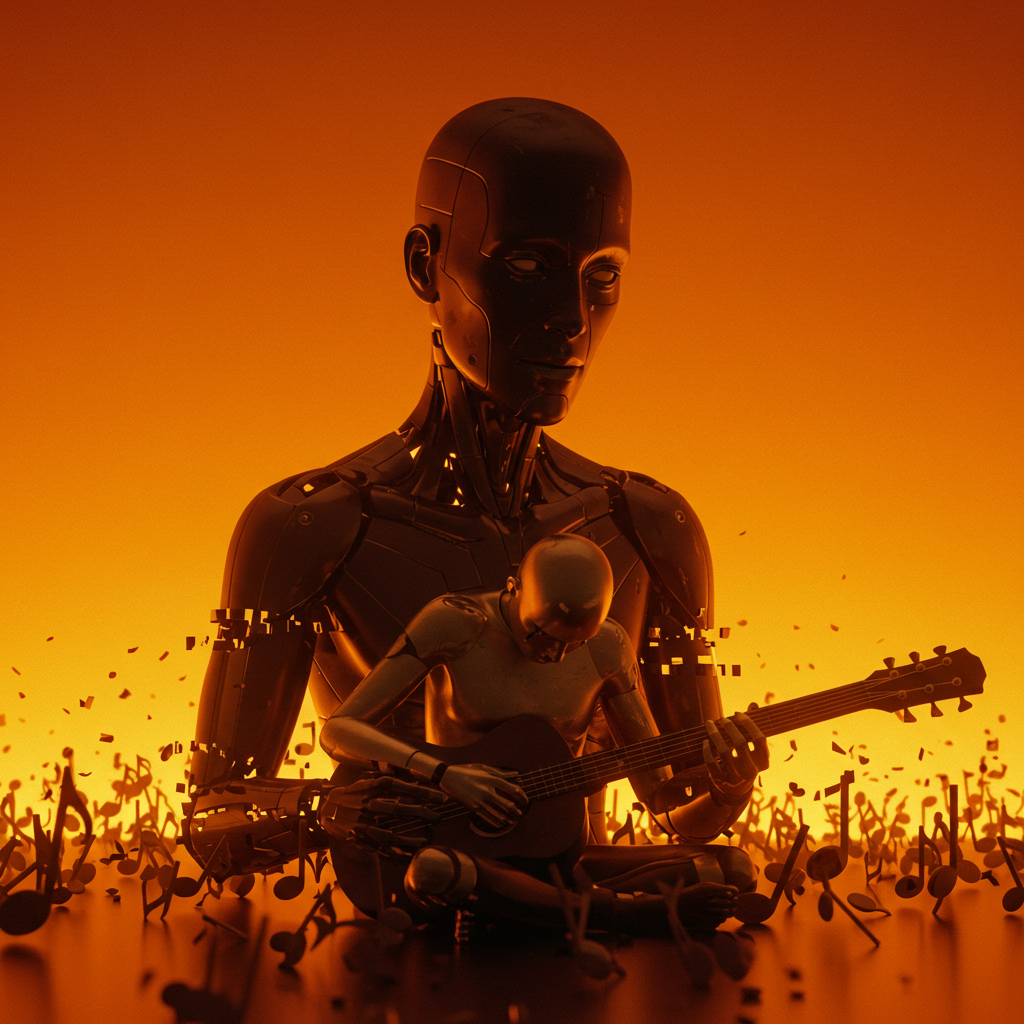
\includegraphics[width=\columnwidth]{graph/ai_risk}
        \end{figure}
    \end{columns}
\end{frame}




%\begin{frame}{music ai}{opportunities \& threats 1/2}
    %\vspace{-5mm}
    %\begin{columns}
    %\column{.65\linewidth}
        %\begin{itemize}
            %\item \textbf{ethical considerations}
                %\begin{itemize}
                    %\item training data (copyright, privacy)
                    %\item responsible system usage
                    %\item addressing bias
                %\end{itemize}
            %\smallskip
            %\item \textbf{economic impact}
                %\begin{itemize}
                    %\item understanding the implications for music professionals
                    %\item adapting to new business models and revenue streams
                %\end{itemize}
            %\smallskip
            %\item   \textbf{quality and authenticity}
                %\begin{itemize}
                    %\item plagiarism
                    %\item balancing novelty and predictability/homogeneity
                    %\item hallucination
                %\end{itemize}
            %\smallskip
        %\end{itemize}
    %\column{.35\linewidth}
        %\vspace{20mm}
        %\begin{figure}%
            %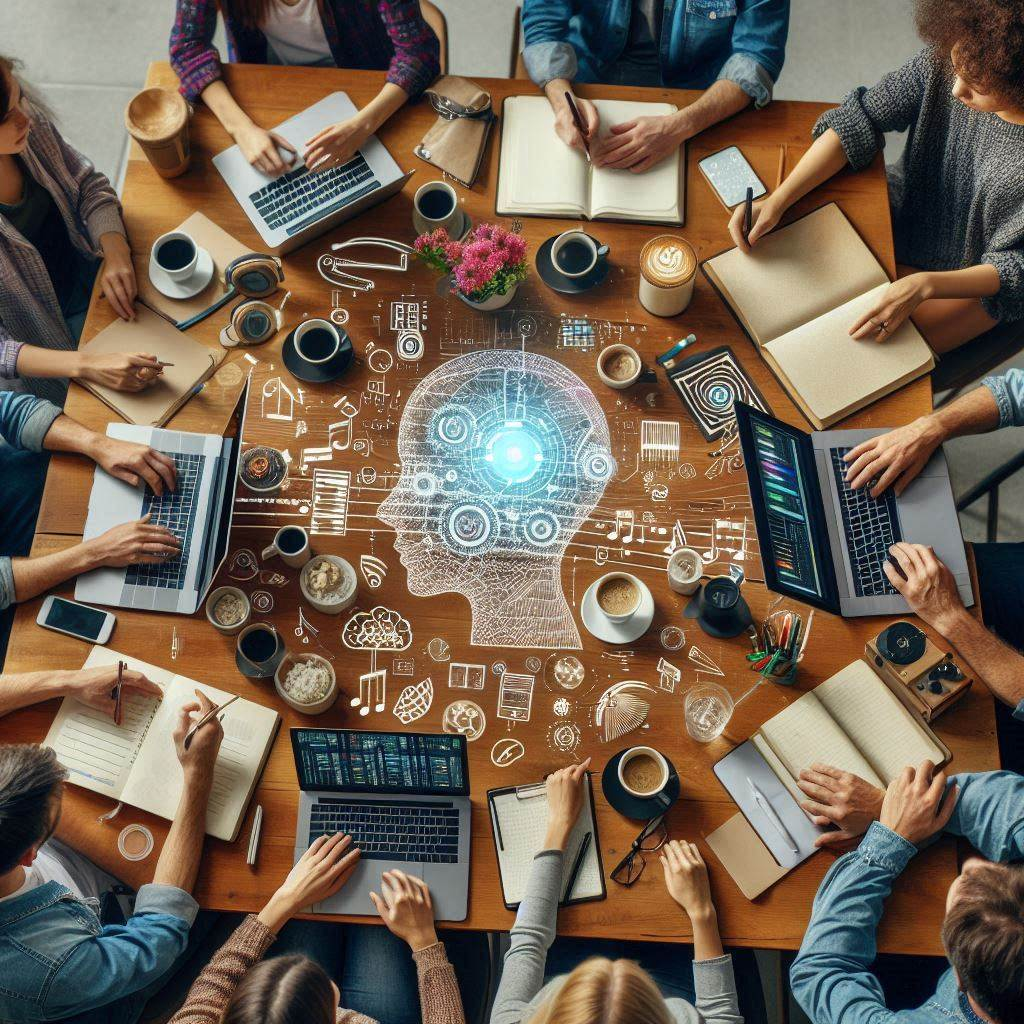
\includegraphics[width=.8\columnwidth]{responsible-ai}%
        %\end{figure}
    %\end{columns}
%\end{frame}
%
%\begin{frame}{challenges}{challenges in (music) ai 2/2}
    %\vspace{-5mm}
    %\begin{columns}
    %\column{.65\linewidth}
        %\begin{itemize}
            %\item   \textbf{sustainability}
                %\begin{itemize}
                    %\item energy consumption
                %\end{itemize}
            %\smallskip
            %\item   \textbf{ownership and copyright}
                %\begin{itemize}
                    %\item protecting rights of content creators while democratizing the creative process
                    %\item navigating complex copyright laws
                    %\item accountability \& liability
                %\end{itemize}
            %\smallskip
            %\item   \textbf{regulatory framework}
                %\begin{itemize}
                    %\item fair use terms
                    %\item transparency and interpretability
                    %\item labeling of ai-created content
                    %\item public perception
                %\end{itemize}
        %\end{itemize}
    %\column{.35\linewidth}
        %\vspace{20mm}
        %\begin{figure}%
            %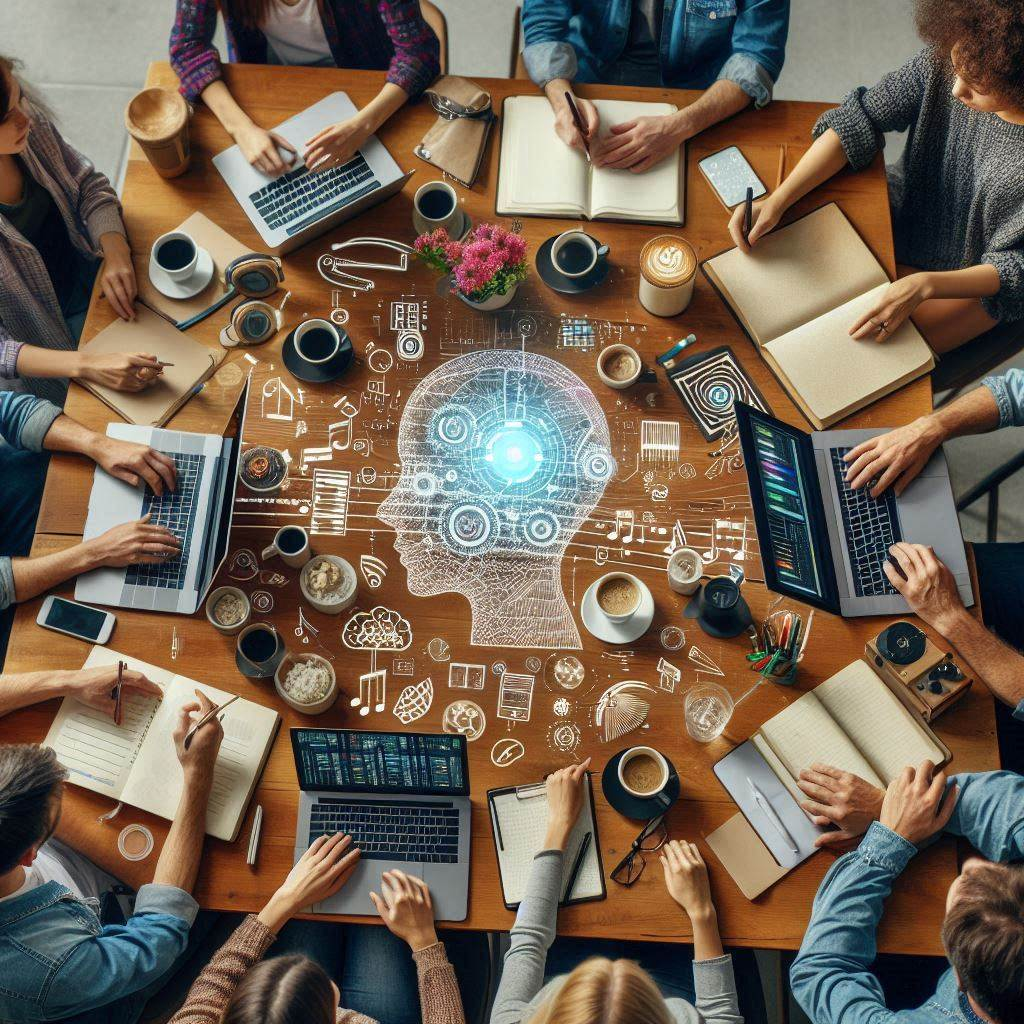
\includegraphics[width=.8\columnwidth]{responsible-ai}%
        %\end{figure}
    %\end{columns}
%\end{frame}
